\documentclass[12pt]{extarticle}
\usepackage[utf8]{inputenc}
\usepackage{cite}
\usepackage[top=1in, bottom=1in, left=1.2in, right=1.2in]{geometry}
\usepackage{booktabs}
\usepackage{graphicx}
\usepackage{amsmath}
\usepackage{amssymb}
\usepackage{hyperref}
\usepackage{enumitem}
\usepackage{longtable}
\usepackage{array}
\usepackage{multirow}
\usepackage{float}

\title{\vspace{-4em} BetaSpray: Climbing Route Visualization System \\ \large Design Document}
\author{Prakhar Gupta (\texttt{prakhar7}), Ingi Helgason (\texttt{ingih2}),\\ Maxwell Beach (\texttt{mlbeach2})}
\date{ECE 445 --- Spring 2026}

\begin{document}

\maketitle
\tableofcontents
\newpage

% =============================================================================
\section{Introduction}
% =============================================================================

\subsection{Problem and Solution}

Spray walls are a popular fixture in modern climbing gyms, consisting of a dense grid of holds
mounted on a single wall surface. Unlike pre-set routes marked with colored tape, spray walls
allow climbers to define their own routes by choosing any subset of holds. This flexibility
makes spray walls an excellent training tool, but it introduces a significant usability problem:
there is no practical way to record, recall, or share a custom route once a climber steps off
the wall.

Currently, climbers must memorize which holds belong to a given route or resort to taking
photographs and manually annotating them. This process is error-prone, time-consuming, and does
not scale. In a training environment, inconsistent route recall leads to unreliable progression
tracking. In a community setting, the inability to easily share routes limits the collaborative
potential of spray walls. The International Federation of Sport Climbing (IFSC) has noted the
growing importance of structured training tools for competitive climbing~\cite{ifsc}, and
existing commercial solutions such as the Kilter Board and MoonBoard address this need only for
proprietary, purpose-built walls with integrated LEDs---not for the far more common generic
spray walls found in most gyms~\cite{moonboard}.

BetaSpray is a standalone device that scans a spray wall, identifies individual holds, and uses
servo-actuated laser pointers to visually highlight route-specific holds in real time. The
system consists of three main subsystems: a \textbf{vision mapping subsystem} that captures
images of the wall and detects hold positions using an OV5640 camera module and a computer
vision pipeline running on the ESP32-S3, a \textbf{projection subsystem} that directs laser
beams onto target holds via 2-axis servo gimbals, and a \textbf{user interface subsystem} that
allows climbers to create, store, and replay routes through a web application hosted on the
ESP32-S3. A \textbf{power subsystem} provides regulated 5\,V and 3.3\,V rails to all
components.

The device is designed to sit on the floor in front of a spray wall, powered from a standard
wall outlet. The camera captures the wall layout, hold positions are extracted and stored, and
when a route is selected the laser gimbals sequentially illuminate the corresponding holds.
Routes are stored locally on the ESP32 via the integrated 16\,MB QSPI flash, and the lightweight HTTP server allows
wireless route management from a phone or laptop. The PCB footprint is approximately
10\,cm~$\times$~10\,cm, designed to fit within the overall device enclosure.

\subsection{Visual Aid}

\begin{figure}[H]
    \centering
    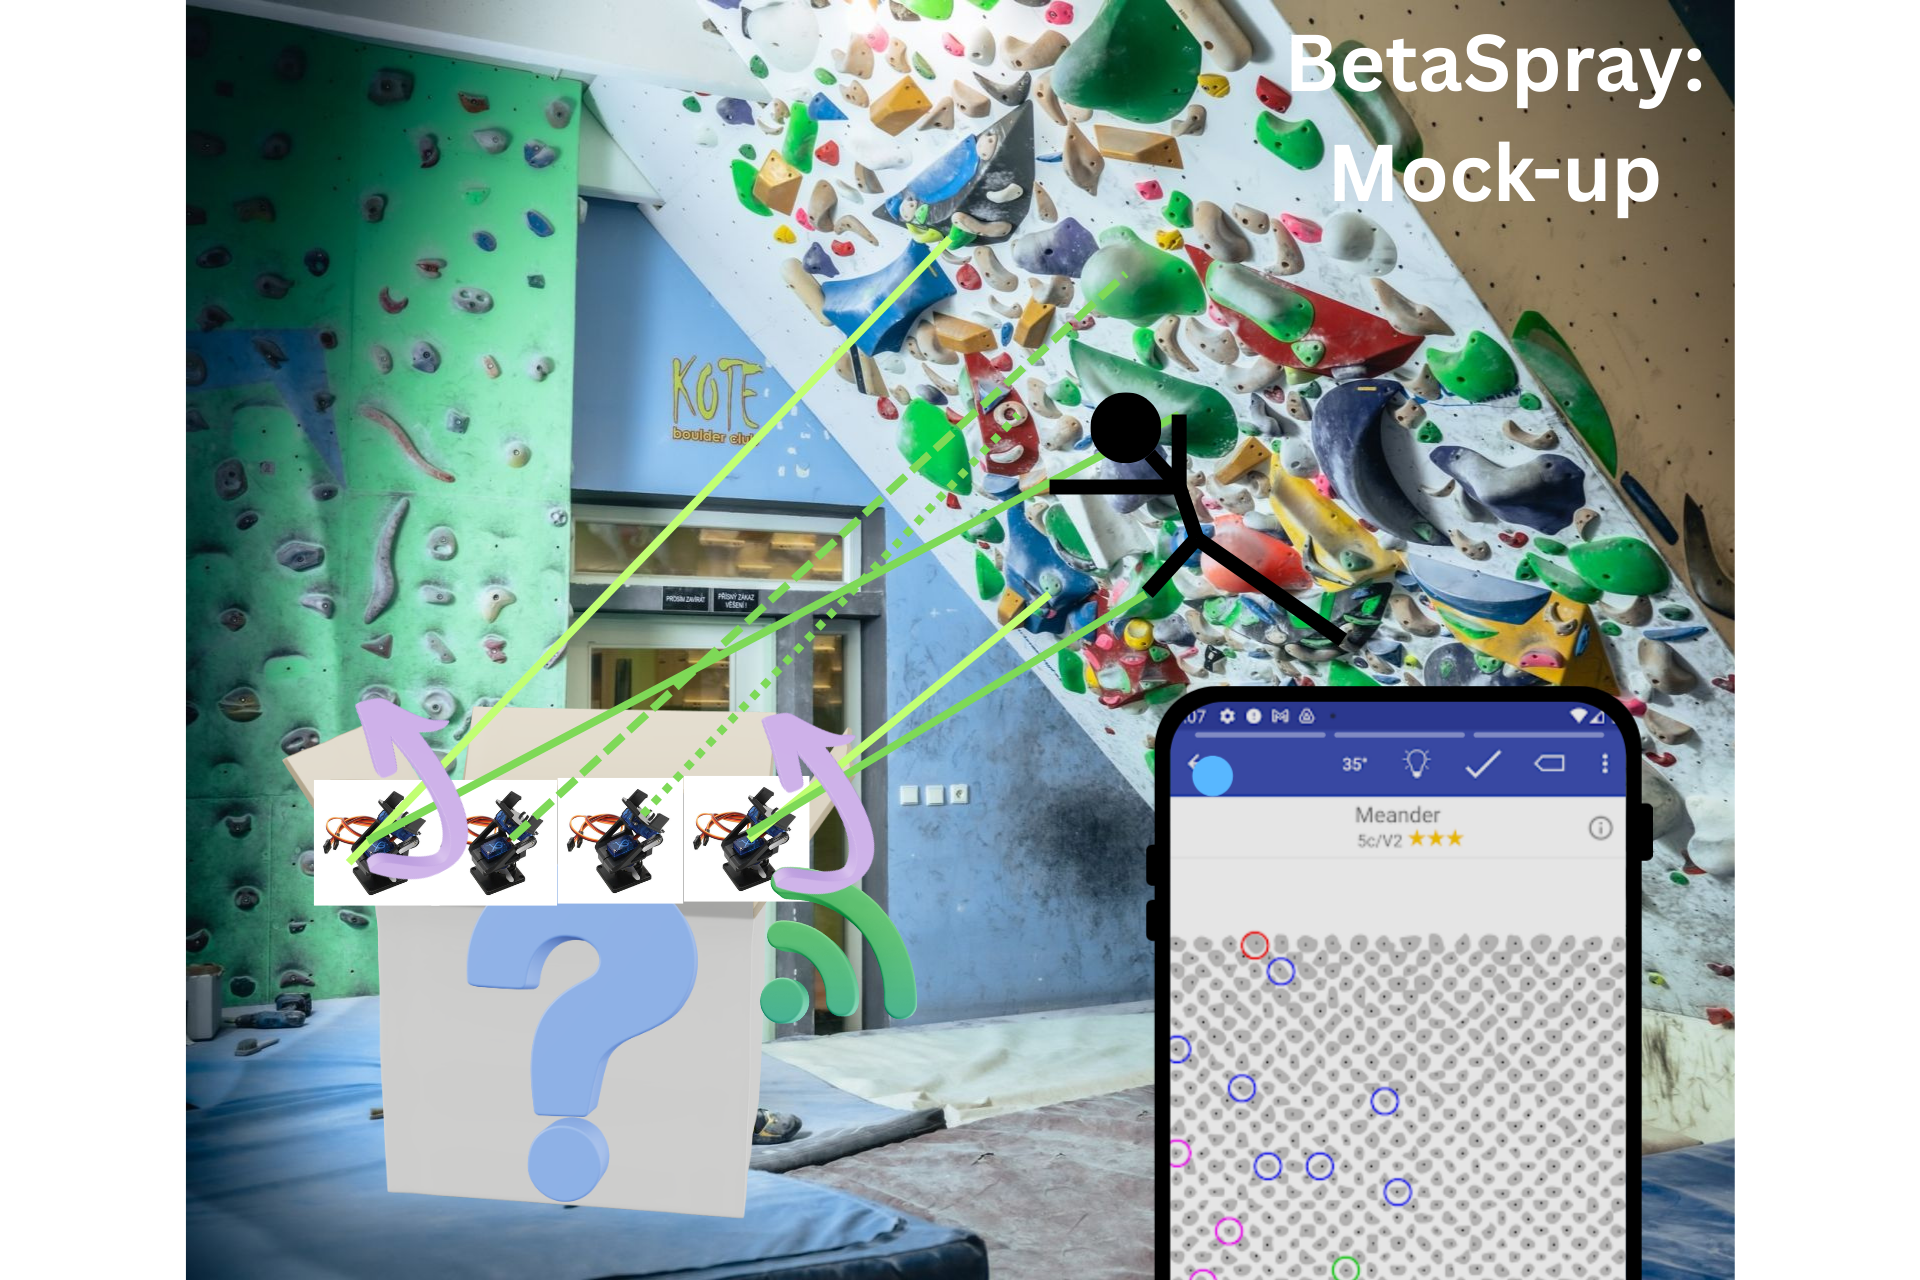
\includegraphics[width=0.9\linewidth]{img/mockup.png}
    \caption{BetaSpray in use: the device sits on the floor in front of a spray wall. The
    camera scans the wall and a phone or laptop connects over Wi-Fi to select a route, after
    which the servo-actuated laser gimbals illuminate the relevant holds.}
    \label{fig:visual_aid}
\end{figure}

\subsection{High-Level Requirements}

\begin{enumerate}
    \item The laser projection subsystem shall direct each laser pointer to its target hold with
          a positional accuracy of $\pm$5\,cm at a projection distance of 3\,m, sufficient to
          unambiguously identify individual holds on a standard spray wall.

    \item The vision mapping subsystem shall detect and localize at least 90\% of holds on a
          spray wall under standard gym lighting conditions ($\geq$300\,lux) within 30 seconds
          of initiating a scan.

    \item The user interface subsystem shall allow a user to create, save, and replay a route
          with an end-to-end response latency of less than 200\,ms from command input to first
          laser actuation.

    \item All laser modules shall be Class~2 ($<$1\,mW continuous visible output) to comply
          with IEC~60825-1 eye safety requirements~\cite{iec60825}.
\end{enumerate}

% =============================================================================
\newpage
\section{Design}
% =============================================================================

\subsection{Block Diagram}

\begin{figure}[H]
    \centering
    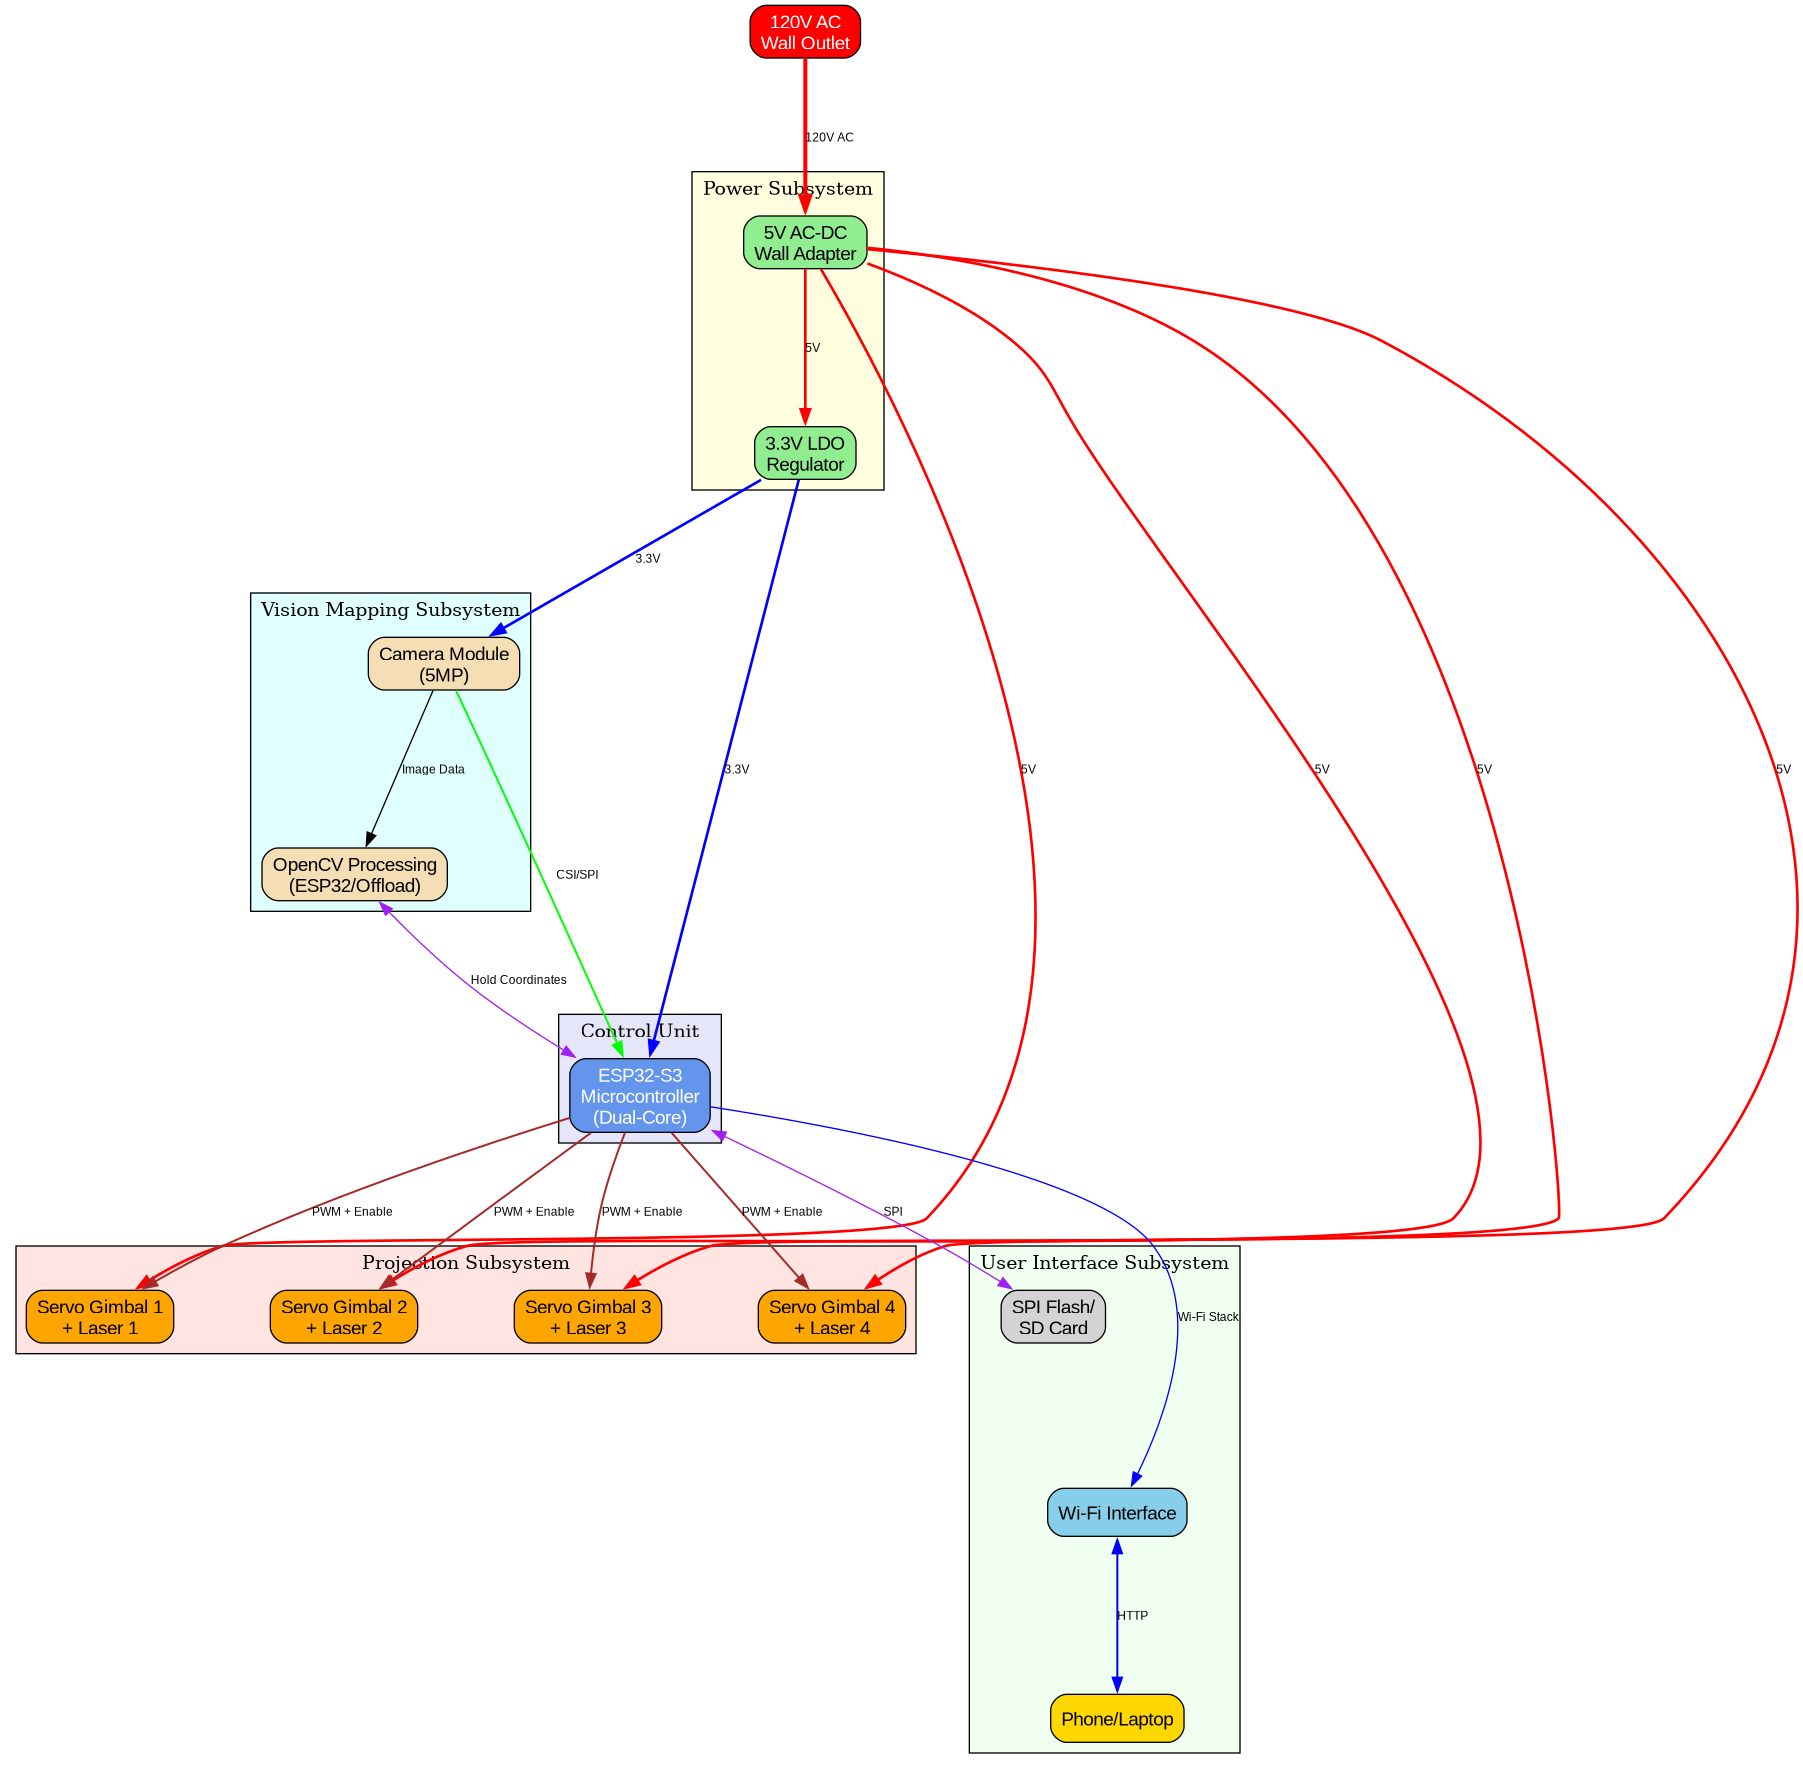
\includegraphics[width=0.85\linewidth]{img/block_diagram.png}
    \caption{Top-level block diagram of the BetaSpray system. Voltage rails (5\,V, 3.3\,V) and
    data buses (DVP, PWM, SPI, I$^2$C, Wi-Fi) are labeled on each inter-subsystem connection.}
    \label{fig:blockdiagram}
\end{figure}

The system centers on the ESP32-S3 microcontroller, which orchestrates all four subsystems.
The power subsystem converts mains power to 5\,V and 3.3\,V rails. The vision mapping
subsystem feeds raw camera frames into the ESP32-S3 over an 8-bit DVP parallel bus. The
projection subsystem receives PWM commands from the ESP32-S3 to drive up to four 2-axis servo
gimbals. The user interface subsystem communicates with client devices over 802.11 Wi-Fi using
a lightweight HTTP server. Route data is persisted on the 16\,MB QSPI flash integrated in the
ESP32-S3-WROOM-1-N16R8 module~\cite{esp32s3_wroom_ds}.

% TODO: Regenerate or update block_diagram.png to reflect OV5640 (DVP), confirmed servo count
% (4×), and SPI flash storage. Label all voltage rails and data buses clearly.

\subsection{Physical Design}

% TODO: Add dimensioned drawing or CAD render of the enclosure showing:
%   - PCB location (~10 cm × 15 cm, with 1/8 in mounting holes, 1/4 in from corners)
%   - Camera module placement and field-of-view cone
%   - Four servo gimbal positions and laser exit apertures
%   - Power inlet (USB-C or barrel jack) location
%   - Overall device envelope (target ≤ 25 cm × 25 cm footprint, ≤ 40 cm height)

The BetaSpray device is designed to rest on the floor in front of the spray wall. The PCB
measures approximately 10\,cm~$\times$~15\,cm and mounts to the enclosure base via four
1/8\,in mounting holes located 1/4\,in from each corner. The OV5640 camera module is elevated
and angled to cover the full wall extent from the floor-level vantage point. The four laser
gimbals are arranged in a horizontal row with sufficient spacing to avoid mechanical
interference at the extremes of their angular travel ($\pm$90$^\circ$ per axis).

\subsection{Power Subsystem}

\subsubsection{Design}

The power subsystem converts a standard 5\,V USB-C wall adapter output into the two rails
required by the system. A 3.3\,V low-dropout (LDO) linear regulator (e.g., AMS1117-3.3 or
equivalent) steps the 5\,V rail down for the ESP32-S3, OV5640 camera, servo motors, and
logic-level peripherals. Laser modules operate directly from the 5\,V rail.

Decoupling capacitors are placed at every power consumer: 100\,$\mu$F bulk electrolytic
capacitors on the 5\,V and 3.3\,V rails to absorb low-frequency transients from servo PWM
switching (servos draw peak current on the 3.3\,V rail), and 100\,nF ceramic capacitors at
each IC supply pin for high-frequency noise suppression. The USB-C port provides power
connectivity, as well as supports JTAG programming of the microcontroller using the 
data lines.

% TODO: @INGI Add schematic screenshot of power subsystem from KiCad (power_subsystem.kicad_sch)
% TODO: @INGI Add hand-calculation showing LDO output stability under 1 A step load

\subsubsection{Flowchart}

\begin{figure}[H]
\centering
\fbox{\begin{minipage}[c][6cm][c]{0.88\linewidth}
\centering\small\textit{--- Power subsystem flowchart ---}
\end{minipage}}
\caption{Power subsystem flowchart.}
\label{fig:flow-power}
\end{figure}

\subsubsection{State Machine}

\begin{table}[H]
\small\centering
\begin{tabular}{>{\raggedright}p{0.13\linewidth}
                >{\raggedright}p{0.28\linewidth}
                >{\raggedright}p{0.13\linewidth}
                >{\raggedright\arraybackslash}p{0.33\linewidth}}
\toprule
\textbf{State} & \textbf{Event / Guard} & \textbf{Next State} & \textbf{Action} \\
\midrule
OFF   & Power applied                  & BOOT  & Enable LDO; start rail-settle timer \\
BOOT  & Rails within spec              & RUN   & Assert power-good signal to ESP32 \\
RUN   & Power stability issue detected & FAULT & De-assert power-good; log fault \\
FAULT & Fault cleared                  & BOOT  & Re-enable LDO; restart settle timer \\
\bottomrule
\end{tabular}
\caption{Power subsystem FSM.}
\label{tab:fsm-power}
\end{table}

\subsubsection{Requirements and Verifications}

\begin{longtable}{>{\raggedright\arraybackslash}p{0.45\linewidth}
                  >{\raggedright\arraybackslash}p{0.45\linewidth}}
\toprule
\textbf{Requirement} & \textbf{Verification} \\
\midrule
\endhead
\bottomrule
\endfoot

%% TODO: @INGI. Check this

The 5\,V rail must supply sufficient current to power the LDO input and laser modules
continuously. &
Measure rail voltage with a DMM while all lasers are enabled and the LDO is under full load.
Verify rail stays within $5\,\text{V} \pm 0.25\,\text{V}$. \\
\addlinespace

The 3.3\,V LDO output must supply at least 1.5\,A continuously while all servos, camera, and
microcontroller are active, and must remain within $\pm$0.1\,V during servo-induced load
transients. &
Measure 3.3\,V rail with a DMM at full load (4 servos stall, camera streaming, MCU Wi-Fi
active). Verify within $3.3\,\text{V} \pm 0.1\,\text{V}$. Capture the rail on an
oscilloscope during a simultaneous 4-servo step; verify peak deviation $<100\,\text{mV}$. \\
\addlinespace


The 100\,$\mu$F bulk capacitors on both rails must suppress PWM switching ripple to
$<$50\,mV\,pk-pk under normal load. &
Measure rail ripple on an oscilloscope (AC coupled, 20\,MHz BW limit) during PWM operation.
Verify ripple $<50\,\text{mV}$\,pk-pk. \\
\end{longtable}

% =============================================================================
\subsection{Vision Mapping Subsystem}
% =============================================================================

\subsubsection{Design}

The vision mapping subsystem is responsible for scanning the spray wall and detecting the
positions of climbing holds. An OV5640 camera module (5\,MP, up to 2592$\times$1944) with
autofocus communicates with the ESP32-S3 via an 8-bit DVP (Digital Video Port) parallel
interface. The DVP signals---8 pixel-data lines (D2--D9), HREF, VSYNC, PCLK---are routed to
dedicated ESP32-S3 camera-interface GPIO pins avoiding strapping pins (GPIO0, 3, 45, 46),
PSRAM SPI pins (GPIO35--37), and USB pins (GPIO19--20). Camera configuration is handled over
I$^2$C (SCCB protocol) on a bus. While I$^2$C supports sharing a bus between different devices,
we only use the OV5640 and the ESP in this case.

The external XCLK line is left unconnected; the
OV5640 uses its internal 24\,MHz oscillator.

The wall-scanning pipeline proceeds in four stages:
\begin{enumerate}
    \item \textbf{Capture:} Trigger the OV5640 and read one full-resolution frame over DVP.
    \item \textbf{Flash save:} Write the raw frame as a file on the FatFS volume (e.g.\
    \texttt{/img/wall.raw}). This decouples capture from processing and allows CV to be
    re-run without recapturing.
    \item \textbf{Hold detection:} Load the saved frame; undistort using a stored lens
    calibration matrix; convert to HSV; apply color thresholding and Canny edge detection to
    locate hold contours. Discard contours below a minimum area threshold.
    % TODO: document HSV threshold ranges and min-area filter values after calibration
    \item \textbf{Angular coordinate extraction:} Convert each detected hold centroid from
    pixel coordinates to angular coordinates $(\phi_i, \theta_i)$ using the geometric model
    in Section~\ref{sec:projection}. Write the complete angular coordinate list to a FatFS
    file (e.g.\ \texttt{/holds.json}).
\end{enumerate}

Post-MVP, \textsc{watch} mode uses the same camera to detect whether the climber is
contacting the currently highlighted hold; see the state machine below.

% TODO: Add example output image showing detected hold contours overlaid on a wall photo
% TODO: Document OpenCV function calls and parameters selected during testing

\subsubsection{Flowchart}

\begin{figure}[H]
\centering
\fbox{\begin{minipage}[c][8cm][c]{0.88\linewidth}
\centering\small\textit{--- Vision mapping flowchart (capture $\to$ flash save $\to$ hold detection $\to$ angular coord extraction) ---}
\end{minipage}}
\caption{Vision mapping subsystem flowchart.}
\label{fig:flow-vision}
\end{figure}

\subsubsection{State Machine}

MVP path: IDLE $\to$ CAPT $\to$ SAVE $\to$ PROC $\to$ READY.
Post-MVP adds \textsc{watch} mode for climber detection and auto-advance.

\begin{table}[H]
\small\centering
\begin{tabular}{>{\raggedright}p{0.13\linewidth}
                >{\raggedright}p{0.28\linewidth}
                >{\raggedright}p{0.13\linewidth}
                >{\raggedright\arraybackslash}p{0.33\linewidth}}
\toprule
\textbf{State} & \textbf{Event / Guard} & \textbf{Next State} & \textbf{Action} \\
\midrule
IDLE  & \texttt{scan\_req}                            & CAPT  & Trigger OV5640 frame capture \\
CAPT  & Frame ready                                   & SAVE  & Write raw frame to SPI flash image partition \\
SAVE  & Write complete                                & PROC  & Run CV pipeline on flash image \\
PROC  & Holds found ($N \geq 1$)                      & READY & Convert centroids to $(\phi_i,\theta_i)$; save coord list to flash \\
PROC  & Detection failed                              & IDLE  & Log error; emit \texttt{scan\_failed} \\
READY & \texttt{scan\_req}                            & CAPT  & Re-trigger capture \\
READY & \texttt{get\_holds()}                         & READY & Return angular coord list to caller \\
\midrule
\multicolumn{4}{l}{\textit{Post-MVP: climber detection}} \\
\midrule
READY & \texttt{watch\_start(hold\_id)}               & WATCH & Load target $(\phi,\theta)$ from coord list; start frame loop \\
WATCH & Frame ready, climber not on hold              & WATCH & Continue monitoring \\
WATCH & Frame ready, climber on hold $\pm\varepsilon$ & WATCH & Emit \texttt{hold\_reached}; load next target \\
WATCH & \texttt{watch\_stop}                          & READY & Stop frame loop \\
\bottomrule
\end{tabular}
\caption{Vision mapping subsystem FSM.}
\label{tab:fsm-vision}
\end{table}

\subsubsection{Requirements and Verifications}

\begin{longtable}{>{\raggedright\arraybackslash}p{0.45\linewidth}
                  >{\raggedright\arraybackslash}p{0.45\linewidth}}
\toprule
\textbf{Requirement} & \textbf{Verification} \\
\midrule
\endhead
\bottomrule
\endfoot

The camera module must capture images at a minimum resolution of 2592$\times$1944 (5\,MP) to
resolve individual holds at distances up to 4\,m. &
Capture a test image at maximum resolution and verify the JPEG header reports
$2592\times1944$. Visually confirm individual 10\,cm holds are distinguishable at 4\,m. \\
\addlinespace

The hold detection algorithm must correctly identify at least 90\% of holds on a standard
spray wall under gym lighting ($\geq$300\,lux). &
Place 20 reference holds on the test wall. Run the detection pipeline and count detected holds.
Repeat 5 times; average detection rate must be $\geq$90\%. \\
\addlinespace

The full wall scan and hold detection pipeline must complete within 30\,s of initiating a
scan. &
Time the pipeline from scan trigger to hold-list output using ESP32-S3 microsecond timestamps.
Verify completion $\leq$30\,s in 5 consecutive runs. \\
\addlinespace

Each detected hold coordinate must be accurate to within $\pm$2\,cm in the wall plane. &
Compare pipeline-reported hold positions to manually measured ground-truth positions for 10
reference holds. Verify all errors $\leq$2\,cm. \\
\addlinespace

During playback, laser spot positions must be detected and reported to the projection subsystem
at $\geq$5\,Hz with position accuracy $\leq$3\,cm. &
Command the gimbal to a fixed angle. Log camera-reported laser position at 10\,Hz. Verify
update rate $\geq$5\,Hz and spot localization error $\leq$3\,cm against a ruler on the wall. \\
\end{longtable}

% =============================================================================
\subsection{Projection Subsystem}
\label{sec:projection}
% =============================================================================

\subsubsection{Design}

The projection subsystem visually marks route holds using laser pointers mounted on 2-axis
servo gimbals. Up to four gimbals are each driven by two PWM signals from the ESP32-S3
(50\,Hz, 1--2\,ms pulse width). SG90 micro servos provide $\geq$180$^\circ$ travel on each
axis with a resolution of $\approx$1$^\circ$/step and are powered from the 3.3\,V rail.
Class~2 KY-008 laser modules ($<$1\,mW red, 650\,nm) are enabled or disabled via
GPIO-driven MOSFETs.

\paragraph{Coordinate Transform.}
To command the gimbal to illuminate wall position $(X_w, Y_w)$ (in cm, wall-plane coordinates
with origin at the wall's lower-left corner), we compute the required azimuth $\phi$ and
elevation $\theta$ from the gimbal's known position $(x_g, y_g, z_g)$ relative to the wall:

\begin{align}
    \Delta X &= X_w - x_g, \quad \Delta Y = Y_w - y_g, \quad \Delta Z = z_g \\
    \theta   &= \arctan\!\left(\frac{\Delta Y}{\sqrt{\Delta X^2 + \Delta Z^2}}\right) \\
    \phi     &= \arctan\!\left(\frac{\Delta X}{\Delta Z}\right)
\end{align}

Angles $(\phi, \theta)$ are converted to PWM pulse widths using the servo's calibrated
angle-to-pulse mapping, stored as a lookup table in flash.

\paragraph{Closed-Loop Vision Correction.}
Because hobby servos do not provide position feedback, we implement a software feedback loop.
After each PWM command, the vision subsystem observes the laser spot and returns the 2D wall
error $(\varepsilon_X, \varepsilon_Y)$ (in cm). A proportional corrective step is applied:

\begin{align}
    \Delta\phi   &\leftarrow \Delta\phi   - K_p \cdot \varepsilon_X \\
    \Delta\theta &\leftarrow \Delta\theta - K_p \cdot \varepsilon_Y
\end{align}

where $K_p$ is a tunable gain. As derived in Section~\ref{sec:tolerance}, two to three
iterations reduce the error below the $\pm$5\,cm threshold. The loop runs at 5--10\,Hz,
limited by camera frame rate.

\paragraph{Open-Loop Fallback (Dead Reckoning).}
If laser spot detection via the camera proves infeasible (e.g., insufficient spot contrast,
processing overhead, or occlusion by the climber), the system operates entirely in Layer~1
using calibrated dead reckoning. At startup each gimbal is driven to a fixed reference angle
pointing at a known wall landmark; all subsequent hold coordinates are computed relative to
this origin using the geometric model. The angle-to-PWM LUT is manually tuned during a
one-time calibration pass and stored on FatFS. This mode requires no camera feedback during
playback and serves as the MVP fallback if vision-based correction cannot be validated in
time.
% TODO: measure and document achievable open-loop accuracy after LUT calibration

% TODO: Add schematic screenshot of servo_subsystem.kicad_sch (MOSFET switching, PWM lines)
% TODO: Add simulation or measured step response of a single gimbal axis

\subsubsection{Flowchart}

\begin{figure}[H]
\centering
\fbox{\begin{minipage}[c][8cm][c]{0.88\linewidth}
\centering\small\textit{--- Projection subsystem flowchart (route load $\to$ coord transform $\to$ PWM HAL $\to$ open-loop / closed-loop correction) ---}
\end{minipage}}
\caption{Projection subsystem flowchart.}
\label{fig:flow-projection}
\end{figure}

\subsubsection{State Machines}

The projection software is organized in three HAL layers plus a route-playback orchestrator.
\textbf{MVP} uses Layer~1 (open-loop) and the Route Playback FSM.
Layer~2 (closed-loop) is activated post-MVP once vision tracking is available.

\paragraph{Layer 0 --- PWM HAL.}
Raw duty-cycle interface to the ESP32-S3 LEDC/MCPWM peripheral.
Exposed as a synchronous API to Layer~1; no asynchronous events.

\begin{table}[H]
\small\centering
\begin{tabular}{>{\raggedright}p{0.13\linewidth}
                >{\raggedright}p{0.28\linewidth}
                >{\raggedright}p{0.13\linewidth}
                >{\raggedright\arraybackslash}p{0.33\linewidth}}
\toprule
\textbf{State} & \textbf{Event / Guard} & \textbf{Next State} & \textbf{Action} \\
\midrule
OFF & \texttt{enable(ch, d)}    & ON  & Configure LEDC timer; write duty \texttt{d} to channel \texttt{ch} \\
ON  & \texttt{set\_duty(ch, d)} & ON  & Update duty register; applies next PWM period \\
ON  & \texttt{disable(ch)}      & OFF & Set duty to 0; stop PWM output \\
\bottomrule
\end{tabular}
\caption{Layer~0: PWM HAL FSM (per channel).}
\label{tab:fsm-pwm-hal}
\end{table}

\paragraph{Layer 1 --- Open-Loop Gimbal.}
Maps target angles $(\phi,\,\theta)$ to duty cycles via a calibration LUT.
\textbf{Used in MVP.}

\begin{table}[H]
\small\centering
\begin{tabular}{>{\raggedright}p{0.13\linewidth}
                >{\raggedright}p{0.28\linewidth}
                >{\raggedright}p{0.13\linewidth}
                >{\raggedright\arraybackslash}p{0.33\linewidth}}
\toprule
\textbf{State} & \textbf{Event / Guard} & \textbf{Next State} & \textbf{Action} \\
\midrule
IDLE  & \texttt{point($\phi$, $\theta$)} & MOVE  & LUT lookup $\to (d_\text{az}, d_\text{el})$; HAL enable+duty; start settle timer \\
MOVE  & Settle timer expired             & HOLD  & Emit \texttt{settled} \\
MOVE  & \texttt{point($\phi$, $\theta$)} & MOVE  & Re-lookup; update HAL duties; reset timer \\
HOLD  & \texttt{point($\phi$, $\theta$)} & MOVE  & LUT lookup; update HAL duties; restart timer \\
HOLD  & \texttt{disable()}               & IDLE  & HAL disable both axes \\
MOVE  & Settle timeout                   & FAULT & HAL disable all; emit \texttt{fault} \\
FAULT & \texttt{reset()}                 & IDLE  & --- \\
\bottomrule
\end{tabular}
\caption{Layer~1: open-loop gimbal FSM (per gimbal).}
\label{tab:fsm-ol-gimbal}
\end{table}

\paragraph{Layer 2 --- Closed-Loop Gimbal (post-MVP).}
Wraps Layer~1; adds vision-feedback correction loop.

\begin{table}[H]
\small\centering
\begin{tabular}{>{\raggedright}p{0.13\linewidth}
                >{\raggedright}p{0.28\linewidth}
                >{\raggedright}p{0.13\linewidth}
                >{\raggedright\arraybackslash}p{0.33\linewidth}}
\toprule
\textbf{State} & \textbf{Event / Guard} & \textbf{Next State} & \textbf{Action} \\
\midrule
IDLE  & \texttt{point($X_w$, $Y_w$)}                               & CMD   & Compute $(\phi,\theta)$; call L1 \texttt{point()} \\
CMD   & L1 \texttt{settled}                                         & OBS   & Request laser spot from vision \\
OBS   & Spot rcvd, $|\varepsilon| > \varepsilon_\text{thr}$         & CORR  & $\phi \leftarrow \phi - K_p\varepsilon_X$; $\theta \leftarrow \theta - K_p\varepsilon_Y$; call L1 \texttt{point()} \\
CORR  & L1 \texttt{settled}                                         & OBS   & Request spot \\
OBS   & Spot rcvd, $|\varepsilon| \leq \varepsilon_\text{thr}$      & DONE  & Hold position \\
DONE  & \texttt{point($X_w$, $Y_w$)}                               & CMD   & Compute new $(\phi,\theta)$; call L1 \texttt{point()} \\
DONE  & \texttt{disable()}                                          & IDLE  & Call L1 \texttt{disable()} \\
OBS   & Vision timeout                                              & FAULT & L1 \texttt{disable()}; emit \texttt{fault} \\
FAULT & \texttt{reset()}                                            & IDLE  & --- \\
\bottomrule
\end{tabular}
\caption{Layer~2: closed-loop gimbal FSM (post-MVP, per gimbal).}
\label{tab:fsm-cl-gimbal}
\end{table}

\paragraph{Route Playback Orchestrator (MVP).}
Drives gimbals through a time-series of holds at a fixed dwell time $T_\text{dwell}$.
MVP: advances on dwell timer (climber follows device pace).
Full: advances on \texttt{hold\_reached} from vision subsystem (climber on hold $\pm\varepsilon$).
Route is a list of angular coordinate pairs $(\phi_i, \theta_i)$ loaded from SPI flash.

\begin{table}[H]
\small\centering
\begin{tabular}{>{\raggedright}p{0.13\linewidth}
                >{\raggedright}p{0.28\linewidth}
                >{\raggedright}p{0.13\linewidth}
                >{\raggedright\arraybackslash}p{0.33\linewidth}}
\toprule
\textbf{State} & \textbf{Event / Guard} & \textbf{Next State} & \textbf{Action} \\
\midrule
IDLE  & \texttt{start(route)}                               & PROJ  & $i \leftarrow 0$; load $(\phi_0,\theta_0)$; \texttt{point()}; laser on; start dwell timer \\
PROJ  & Dwell exp, $i < N-1$ \textsf{[MVP]}                & PROJ  & $i \leftarrow i+1$; load $(\phi_i,\theta_i)$; \texttt{point()}; reset timer \\
PROJ  & Dwell exp, $i = N-1$ \textsf{[MVP]}                & IDLE  & Laser off; emit \texttt{route\_done} \\
PROJ  & \texttt{hold\_reached}, $i < N-1$ \textsf{[full]}  & PROJ  & $i \leftarrow i+1$; load $(\phi_i,\theta_i)$; \texttt{point()} \\
PROJ  & \texttt{hold\_reached}, $i = N-1$ \textsf{[full]}  & IDLE  & Laser off; emit \texttt{route\_done} \\
PROJ  & \texttt{pause()}                                    & PAUSE & Stop dwell timer \\
PAUSE & \texttt{resume()}                                   & PROJ  & Restart dwell timer \\
PAUSE & \texttt{stop()}                                     & IDLE  & Laser off \\
(any) & Gimbal fault                                        & IDLE  & Laser off; emit \texttt{error} \\
\bottomrule
\end{tabular}
\caption{Route playback orchestrator FSM (MVP). $T_\text{dwell}$ configurable.}
\label{tab:fsm-playback}
\end{table}

\subsubsection{Requirements and Verifications}

\begin{longtable}{>{\raggedright\arraybackslash}p{0.45\linewidth}
                  >{\raggedright\arraybackslash}p{0.45\linewidth}}
\toprule
\textbf{Requirement} & \textbf{Verification} \\
\midrule
\endhead
\bottomrule
\endfoot

Each servo gimbal must provide $\geq$180$^\circ$ of rotation on each axis with an open-loop
positioning resolution of $\leq$1$^\circ$. &
Command the servo across its full range in 1$^\circ$ steps using a calibration jig with a
protractor. Verify mechanical travel $\geq$180$^\circ$ and no missed steps. \\
\addlinespace

Each laser module must be Class~2 ($<$1\,mW continuous output at 650\,nm) to comply with
IEC~60825-1. &
Measure laser optical power with a calibrated photodiode power meter. Verify output
$<$1\,mW. \\
\addlinespace

Each laser must produce a visible spot of $\geq$1\,cm diameter at 4\,m to unambiguously
identify the targeted hold. &
Project each laser onto a wall at 4\,m and measure spot diameter with a ruler. Verify
$\geq$1\,cm. \\
\addlinespace

The servo transition time between any two target holds must be $<$500\,ms. &
Command a worst-case angle change ($\geq$90$^\circ$ on both axes simultaneously) and measure
elapsed time from PWM update to mechanical settle using oscilloscope and high-speed camera.
Verify $<$500\,ms. \\
\addlinespace

After closed-loop correction, the laser spot must be within $\pm$5\,cm of the target hold at
3\,m projection distance. &
Command the gimbal to 20 randomly chosen wall coordinates. After correction loop convergence,
measure residual error with a ruler. Verify all 20 errors $\leq$5\,cm. \\
\end{longtable}

% =============================================================================
\subsection{User Interface Subsystem}
% =============================================================================

\subsubsection{Design}

The user interface subsystem enables climbers to manage routes via a web application served
directly by the ESP32-S3. The ESP32-S3 runs an HTTP server using the ESP-IDF networking stack.
Static HTML/CSS/JavaScript files for the web interface are stored in the SPI flash partition.
Route data (angular coordinate lists for selected holds, route names) is stored as JSON files
on a FatFS volume mounted on the integrated 16\,MB QSPI flash of the ESP32-S3-WROOM-1-N16R8.
The device stores a maximum of 5 routes concurrently (e.g.\ \texttt{/routes/r0.json} \ldots
\texttt{/routes/r4.json}). Static web assets are also served from FatFS.
The ESP32-S3 operates as a Wi-Fi access point in standalone mode, enabling use without
external network infrastructure.

The web interface provides four primary workflows:
\begin{enumerate}
    \item \textbf{Scan:} Triggers the vision mapping pipeline and displays the detected hold
    map as an SVG overlay on a wall thumbnail.
    \item \textbf{Create:} Allows the user to click holds on the displayed map to build a route
    and assign it a name.
    \item \textbf{Save:} Serializes the route and writes it to the flash store via a POST
    request.
    \item \textbf{Replay:} Selects a saved route and commands the projection subsystem to
    illuminate holds sequentially.
\end{enumerate}

% TODO: Add UI wireframe / screenshot mockup of the web interface (scan, create, replay views)
% TODO: Document ESP-IDF partition table and FatFS layout:
%   partition table: bootloader, app (OTA), nvs, FatFS data partition
%   FatFS tree: /img/wall.raw, /holds.json, /routes/r{0-4}.json, /www/ (web assets)

\subsubsection{Flowchart}

\begin{figure}[H]
\centering
\fbox{\begin{minipage}[c][6cm][c]{0.88\linewidth}
\centering\small\textit{--- User interface flowchart (boot $\to$ Wi-Fi AP $\to$ HTTP request dispatch $\to$ scan / edit / replay) ---}
\end{minipage}}
\caption{User interface subsystem flowchart.}
\label{fig:flow-ui}
\end{figure}

\subsubsection{State Machine}

The HTTP server is event-driven; FSM state tracks what the system is currently doing.
MVP requires IDLE, SCAN, EDIT, and PLAY states. Max 5 routes on flash.

\begin{table}[H]
\small\centering
\begin{tabular}{>{\raggedright}p{0.13\linewidth}
                >{\raggedright}p{0.28\linewidth}
                >{\raggedright}p{0.13\linewidth}
                >{\raggedright\arraybackslash}p{0.33\linewidth}}
\toprule
\textbf{State} & \textbf{Event / Guard} & \textbf{Next State} & \textbf{Action} \\
\midrule
INIT  & Boot complete                      & IDLE  & Start Wi-Fi AP; start HTTP server \\
IDLE  & \texttt{POST /scan}                & SCAN  & Invoke \texttt{vision::scan()} \\
SCAN  & Scan complete                      & IDLE  & Cache hold map; respond 200 + hold list \\
SCAN  & Scan failed                        & IDLE  & Respond 500 \\
IDLE  & \texttt{POST /route/create}        & EDIT  & Open empty route buffer \\
EDIT  & \texttt{POST /route/hold/\{id\}}   & EDIT  & Append hold to buffer \\
EDIT  & \texttt{POST /route/save}          & IDLE  & Write route to flash; respond 200; respond 409 if 5-route limit reached \\
EDIT  & \texttt{POST /route/discard}       & IDLE  & Clear buffer; respond 200 \\
IDLE  & \texttt{POST /route/\{id\}/replay} & PLAY  & Call \texttt{playback::start(route)}; respond 202 \\
PLAY  & Route complete                     & IDLE  & Notify client \\
PLAY  & \texttt{POST /route/stop}          & IDLE  & Call \texttt{playback::stop()}; respond 200 \\
(any) & Hardware fault                     & FAULT & Laser off; respond 503 on pending requests \\
FAULT & \texttt{POST /reset}               & INIT  & Restart subsystems \\
\bottomrule
\end{tabular}
\caption{User interface subsystem FSM.}
\label{tab:fsm-ui}
\end{table}

\subsubsection{Requirements and Verifications}

\begin{longtable}{>{\raggedright\arraybackslash}p{0.45\linewidth}
                  >{\raggedright\arraybackslash}p{0.45\linewidth}}
\toprule
\textbf{Requirement} & \textbf{Verification} \\
\midrule
\endhead
\bottomrule
\endfoot

The ESP32-S3 HTTP server must respond to client GET and POST requests within 100\,ms under
normal operating conditions. &
Use a browser dev-tools network panel or \texttt{curl} with timing to measure round-trip HTTP
response time for 20 requests. Verify all $\leq$100\,ms. \\
\addlinespace

The system must support storage of at least 50 routes, each containing up to 30 holds, on
SPI flash. &
Create 50 routes of 30 holds each via the API, then verify all are retrievable and correct.
Confirm SPI flash usage does not exceed partition size. \\
\addlinespace

The web interface must be accessible from Chrome, Safari, and Firefox without app installation. &
Load the interface on each browser. Verify all four workflows (scan, create, save, replay)
function correctly. \\
\addlinespace

The Wi-Fi link must remain stable at distances up to 10\,m from the device in a typical gym
environment. &
Connect a client device at 10\,m with $\geq$2 walls between the device and client. Perform
20 HTTP transactions; verify $\leq$1 failure. \\
\addlinespace

End-to-end latency from route-replay command input to first laser actuation must be
$<$200\,ms. &
Instrument the firmware with microsecond timestamps at HTTP request receipt and first PWM
output. Measure latency for 10 replay commands; verify all $\leq$200\,ms. \\
\end{longtable}

% =============================================================================
\subsection{System Integration}

\begin{figure}[H]
\centering
\fbox{\begin{minipage}[c][10cm][c]{0.88\linewidth}
\centering\small\textit{--- System integration flowchart (power-on $\to$ wall scan $\to$ route creation $\to$ route playback, showing data flow between all four subsystems) ---}
\end{minipage}}
\caption{End-to-end system integration flowchart.}
\label{fig:flow-integration}
\end{figure}

\subsection{Tolerance Analysis}
\label{sec:tolerance}
% =============================================================================

The most critical tolerance in the BetaSpray system is the angular accuracy of the
servo-actuated laser gimbals, as a pointing error placing the laser on the wrong hold renders
the system unusable.

\paragraph{Geometric Model.}
Consider a laser gimbal at floor level, horizontal distance $d$ from the wall, pointing at a
hold at height $h$. The required elevation angle is:

\begin{equation}
    \theta = \arctan\!\left(\frac{h}{d}\right)
\end{equation}

A small servo angular error $\Delta\theta$ (rad) produces a wall positional error:

\begin{equation}
    \Delta x = \frac{d}{\cos^2\!\theta} \cdot \Delta\theta
\end{equation}

\paragraph{Worst-Case Open-Loop Error.}
For $d = 3$\,m and $h = 4$\,m (near the top of a standard spray wall),
$\theta = \arctan(4/3) \approx 53.1^\circ$. The SG90 servo has a rated accuracy of
$\approx \pm1^\circ$ ($\Delta\theta = 0.0175$\,rad):

\begin{equation}
    \Delta x = \frac{3}{\cos^2(53.1^\circ)} \cdot 0.0175 \approx \frac{3}{0.360} \cdot 0.0175
    \approx 14.6\,\text{cm}
\end{equation}

This exceeds the $\pm$5\,cm requirement. At a lower angle ($h = 2$\,m, $\theta \approx
33.7^\circ$) the error reduces to $\approx$6.2\,cm---still above spec.

\paragraph{Two-Stage Mitigation.}
\begin{enumerate}
    \item \textbf{Calibration mapping:} After wall scan, the system projects each laser onto
    four known reference points and records the actual versus commanded angle. A correction
    lookup table reduces the effective servo error to $\approx\pm0.5^\circ$.

    \item \textbf{Closed-loop vision feedback:} During playback the camera observes the laser
    spot and computes positional error $(\varepsilon_X, \varepsilon_Y)$. A proportional
    controller applies corrective PWM adjustments, converging in 2--3 iterations. Assuming the
    vision subsystem measures positions to within $\pm$3\,cm, the corrected servo error after
    convergence is $\Delta\theta_{\text{corr}} \approx 0.003$\,rad:
\end{enumerate}

\begin{equation}
    \Delta x_{\text{final}} = \frac{3}{0.360} \cdot 0.003 \approx 2.5\,\text{cm} \quad
    (\leq\, \pm5\,\text{cm}\ \checkmark)
\end{equation}

The calibration procedure adds approximately 30\,s to setup time; the real-time feedback loop
operates at 5--10\,Hz with no perceptible latency during route playback.

\paragraph{Dead-Reckoning Fallback Accuracy.}
If vision-based correction (Stage~2) is unavailable, Stage~1 calibration alone leaves a
residual error of $\approx\pm0.5^\circ$ ($\Delta\theta = 0.00873$\,rad). At the worst-case
angle:
\begin{equation}
    \Delta x_{\text{cal}} = \frac{3}{0.360} \cdot 0.00873 \approx 7.3\,\text{cm}
\end{equation}
This exceeds the $\pm5$\,cm spec but is usable as a degraded-mode fallback, particularly at
lower wall angles. Iterative manual LUT tuning beyond the four-reference-point calibration
can further reduce this error.
% TODO: measure and document achievable open-loop accuracy after full LUT calibration
% TODO: Add plot showing simulated error convergence over correction iterations
% TODO: Extend analysis to azimuth axis ($\phi$) to confirm symmetric behavior

% =============================================================================
\newpage
\section{Cost and Schedule}
% =============================================================================


\subsection{Parts}

\begin{longtable}{p{0.30\linewidth} p{0.18\linewidth} p{0.14\linewidth} c r}
\toprule
\textbf{Description} & \textbf{Manufacturer} & \textbf{Part \#} & \textbf{Qty} & \textbf{Cost} \\
\midrule
\endhead
\bottomrule
\endfoot

ESP32-S3-DevKitC-1 (prototyping)     & Espressif        & ESP32-S3-DevKitC-1   & 1 & \$10.00 \\
ESP32-S3 module (PCB)                 & Espressif        & ESP32-S3-WROOM-1-N16R8 & 1 & \$7.00  \\
OV5640 camera module w/ autofocus     & Arducam          & B0272                & 1 & \$25.00 \\
3.3\,V LDO regulator (AMS1117-3.3)   & AMS              & AMS1117-3.3          & 2 & \$1.00  \\
Class 2 laser diode module (KY-008)   & Generic          & KY-008               & 4 & \$8.00  \\
Micro servo motor (SG90)              & Tower Pro        & SG90                 & 8 & \$16.00 \\
2-axis gimbal kit                     & Generic          & ---                  & 4 & \$20.00 \\
USB-C receptacle (power only)         & GCT              & USB4135-GF-A         & 1 & \$0.80  \\
Resettable PTC fuse 3\,A              & Bourns           & MF-R300              & 1 & \$0.50  \\
Schottky diode (polarity protection)  & ON Semi          & 1N5819               & 1 & \$0.20  \\
Bulk electrolytic cap 100\,$\mu$F     & Panasonic        & ECE-A1HKA101         & 4 & \$2.00  \\
Ceramic cap 100\,nF 0402              & Murata           & GCM155R71C104KA55D   & 20 & \$1.00 \\
% TODO: Add remaining BOM items (resistors, MOSFETs for laser enable, connectors, PCB fab)
\midrule
\textbf{Parts subtotal}               &                  &                      &   & \textbf{\$90.50} \\
% TODO: Update subtotal when BOM is finalized
\end{longtable}


\subsection{Schedule}

\begin{longtable}{p{0.06\linewidth} p{0.38\linewidth} p{0.20\linewidth} p{0.20\linewidth}}
\toprule
\textbf{Week} & \textbf{Tasks} & \textbf{Responsible} & \textbf{Deliverable / Milestone} \\
\midrule
\endhead
\bottomrule
\endfoot

1--2  & Finalize PCB schematic (all subsystems); KiCad DRC clean;
        submit first PCB order round &
        Prakhar (vision schematic), Ingi (power), Max (servo) &
        PCB order submitted \\
\addlinespace
3     & Design document draft; tolerance analysis extension;
        FSM diagrams for each subsystem &
        All & Design Document due \\
\addlinespace
4     & Receive PCB Rev~1; bring up power rails; flash ESP32-S3
        bootloader; verify camera DVP communication &
        Prakhar, Ingi & Power-on test passing \\
\addlinespace
5     & Implement OV5640 driver; capture test frames at full
        resolution; verify SCCB register config &
        Prakhar & Camera streaming at 2592$\times$1944 \\
\addlinespace
6     & Implement CV pipeline (HSV threshold, Canny, homography);
        hold detection on test wall &
        Prakhar, Max & $\geq$90\% hold detection on 20-hold test set \\
\addlinespace
7     & Calibrate servo gimbals; implement coordinate transform;
        open-loop pointing test &
        Max, Ingi & Lasers pointing to $\pm$15\,cm (pre-correction) \\
\addlinespace
8     & Implement closed-loop vision correction; integrate with
        CV pipeline; verify $\pm$5\,cm &
        All & Closed-loop accuracy $\leq$5\,cm \\
\addlinespace
9     & Implement HTTP server; route create/save/replay API;
        web frontend &
        Ingi, Max & Route playback via browser \\
\addlinespace
10    & System integration; end-to-end latency test ($<$200\,ms);
        flash storage stress test (50 routes) &
        All & Mock Demo passing all R\&V \\
\addlinespace
11    & PCB Rev~2 (bug fixes from Rev~1); re-run R\&V suite &
        All & PCB Rev~2 order \\
\addlinespace
12    & Final demo preparation; enclosure assembly; safety
        verification (laser power measurement) &
        All & Final Demo \\
\addlinespace
13    & Final report writing; lab notebook completion &
        All & Final Report due \\
\end{longtable}

% =============================================================================
\newpage
\section{Societal Impact, Standards, Ethics, and Safety}
% =============================================================================

\subsection{Public Health, Safety, and Welfare}

BetaSpray has the potential to make climbing training more accessible and systematic. By
enabling easy route creation and sharing, the system lowers the barrier for beginner climbers
who may otherwise struggle to identify appropriate routes on an unmarked spray wall. Consistent
route recall supports reliable progression tracking, which is particularly valuable for climbers
in rehabilitation or adaptive training programs. The environmental impact of the device is
minimal: it uses low-power components and produces no waste during normal operation.

\subsection{Applicable Standards}

\begin{itemize}
    \item \textbf{IEC~60825-1:2014} --- Safety of laser products. BetaSpray uses Class~2
    ($<$1\,mW) lasers, which comply with this standard. Class~2 lasers are safe for accidental
    short-duration exposure due to the natural blink reflex ($\approx$0.25\,s).

    \item \textbf{FDA 21 CFR Part 1040.10} --- Performance standards for laser products. All
    laser modules will be verified to comply before use.

    \item \textbf{IEEE 802.11} --- The Wi-Fi communication standard implemented by the
    ESP32-S3 for the user interface subsystem.

    \item \textbf{IEC~61000-4} --- Electromagnetic compatibility (EMC). The PCB layout follows
    best practices for EMC (solid ground planes, short high-frequency traces, bypass
    capacitors) to minimize radiated emissions from PWM switching.

    % TODO: Identify any UL or CE certification requirements for the power adapter and enclosure
\end{itemize}

\subsection{IEEE/ACM Code of Ethics}

We will adhere to the IEEE Code of Ethics~\cite{ieee_ethics} throughout development. In
accordance with IEEE Code 1.1, we hold paramount the safety and well-being of the public; this
is reflected in our selection of Class~2 lasers and the software interlock that disables all
lasers when no valid wall target is loaded, preventing uncontrolled emission. We will
accurately represent our design capabilities and document limitations transparently in the
final report (IEEE Code 3.1). All open-source libraries (ESP-IDF, OpenCV) and third-party
hardware designs used in this project will be documented and credited accordingly (IEEE Code
7.8).

\subsection{Electrical and Mechanical Safety}

\begin{itemize}
    \item The device is powered from a 5\,V USB-C wall adapter; no mains voltage is present
    inside the enclosure. All exposed connectors are low-voltage SELV circuits.

    \item A polarity-protection diode and 3\,A resettable PTC fuse are included on the input
    power rail to prevent damage from miswiring or overcurrent.

    \item All PCB traces carrying $>$0.5\,A are sized per IPC-2221 for the maximum expected
    current.

    \item The enclosure has no sharp external edges and includes rubber feet to prevent
    displacement on gym floors. Since the device operates in an environment where people are
    physically active, the enclosure must withstand incidental contact without exposing
    internal electronics.

    \item Laser apertures in the enclosure are sized to limit the accessible emission angle,
    further reducing stray beam exposure risk.

    \item All development, soldering, PCB assembly, and high-current testing will be conducted
    in designated ECE~445 laboratory areas in compliance with ECEB lab safety
    standards~\cite{ece445safety}.
\end{itemize}

% =============================================================================
\newpage
\begin{thebibliography}{9}

\bibitem{ifsc}
International Federation of Sport Climbing, ``IFSC Rules 2024,'' \textit{ifsc-climbing.org}.
Accessed: Feb.\ 12, 2026.

\bibitem{moonboard}
Moon Climbing, ``MoonBoard,'' \textit{moonboard.com}. Accessed: Feb.\ 12, 2026.

\bibitem{iec60825}
International Electrotechnical Commission, ``IEC 60825-1: Safety of laser products --- Part 1:
Equipment classification and requirements,'' Ed.\ 3.0, 2014.

\bibitem{ieee_ethics}
IEEE, ``IEEE Code of Ethics,'' \textit{ieee.org},
\url{https://www.ieee.org/about/corporate/governance/p7-8.html}. Accessed: Feb.\ 12, 2026.

\bibitem{ece445safety}
ECE 445 Safety Guidelines, ``Safety --- ECE 445 Senior Design Laboratory,''
\url{https://courses.grainger.illinois.edu/ece445/guidelines/safety.asp}. Accessed:
Feb.\ 12, 2026.

% TODO: Add citation for OV5640 datasheet
% TODO: Add citation for ESP32-S3 Technical Reference Manual
% TODO: Add citation for OpenCV documentation / relevant CV algorithm papers

\end{thebibliography}

\end{document}
